\documentclass[11pt,a4paper]{article}
\usepackage[T1]{fontenc}
\usepackage{lmodern,amsmath,amssymb,amsthm,booktabs,microtype,graphicx}
\usepackage[margin=24mm]{geometry}
\usepackage[colorlinks=true,urlcolor=blue,linkcolor=blue]{hyperref}
\newcommand{\Js}{\mathcal J_s}
\newcommand{\E}{\mathbb E}
\newcommand{\tr}{\operatorname{tr}}
\newcommand{\av}[1]{\langle #1\rangle}
\newcommand{\W}{\mathcal W}
\newcommand{\JH}{\mathsf J_H}
\newcommand{\DD}{\mathfrak D}
\DeclareMathOperator{\sech}{sech}
\title{Closing the cubic singlet two-point spectrum\\A charged covariance lift for the linear residual}
\author{Alan Day \and Chengheng\thanks{AI research assistant (OpenAI).}}
\date{Local research note --- 6 November 2026}
\begin{document}\maketitle
\begin{abstract}
The remaining linear--quadratic and linear--cubic cross spectra can be
tested using the existing embedded-ensemble covariance bridge. The
necessary extra step is a charge-dependent lift of a $(p-1)$-body
ensemble to a $p$-body operator. We give its exact covariance and
marked-product identities. A single centered filter then cancels in
every fixed-degree mixed moment. Together with the preceding
cubic--quadratic cancellation, this closes the positive two-energy
measure of the conserved-subtracted cubic derivative insertion. Its
small-coupling normalized time correlation is a definite combination
of $\sech^6$ and $\sech^4$, rather than the isolated cubic-primary kernel.
\end{abstract}
\section{The completed two-point object}
Use standard CAR, a complex Gaussian $p$-body Hamiltonian $H=H_s$
with overlapping index sets included, and the annealed normalized
trace at $\beta=\mu_{\rm chem}=0$. Set $\hbar=1$, $L=[H,\cdot]$,
$\JH B=\{H,B\}/2$, and first take
\[
 N,p\to\infty,\qquad\lambda=p^2/N>0,\qquad
 q=e^{-4\lambda},\qquad \sigma^2=\Js^2/\lambda.
\]
The preceding notes \cite{local} constructed the linear residual $F$,
quadratic singlet $Y$, and cubic residual $R$. Their diagonal
two-energy measures have the known Mehler weights $q,q^2,q^3$.
We prove the remaining off-diagonal statements
\begin{equation}
 \boxed{d\nu_{FY}=d\nu_{FR}=0\quad\hbox{in DS}.}\label{cross}
\end{equation}
Along with the previous $d\nu_{RY}=0$, these diagonalize the
\emph{two-point} spectral matrix. They do not imply independence
of the operators at higher point order.

For $M_3=\sum_i c_i^\dagger L^3c_i$, subtract the conserved
polynomial $P_N$ defined below. Its complete limiting measure is
\begin{equation}
 \boxed{d\nu_{UU^\dagger}=
 V_F\,d\mu_q+V_R\,d\mu_{q^3}
 +W\left[a\frac{E+E'}2+\frac32(E-E')\right]^2d\mu_{q^2},}
 \label{measure}
\end{equation}
where $U=M_3-P_N$, each $\mu_r$ has unit mass, and $a,V_F,V_R,W$
are specified in Sec.~5. The formula retains the non-Hermitian
time descendant of the actual insertion. It is positive and fixes
all its two-energy moments and every fixed-time two-point function.

\newpage
\section{An operator $L^2$ bridge, not only a covariance estimate}
In charge sector $m$ let $H=\sum_\nu H_\nu$ be the irreducible
rank decomposition, $C=\av{H^2}_m$, and
$\av{H_\nu^2}_m=C\omega_\nu^{(p)}$. Put $h=H/\sqrt C$,
$V_{F,N}=\av{F^2}_m$, $y=F/\sqrt{V_{F,N}}$. The preceding
rank formulas give, with $s=p-\nu$,
\begin{align}
 R_1(s)&=\frac{\omega_{p-s}^{(p-1)}}{\omega_{p-s}^{(p)}}
 =\frac{s(N-2p+s+1)(N-m+p)}{(m-p+1)p^2},\label{ratio}\\
 \widehat y&=\sqrt\lambda\sum_\nu[R_1(p-\nu)-1]h_\nu,
 &\|y-\widehat y\|_2&\longrightarrow0.\label{l2}
\end{align}
Indeed $s$ tends to $\operatorname{Pois}(\lambda)$, the normalized
$F$ filter tends to $(s-\lambda)/\sqrt\lambda$, and
$R_1(s)\to s/\lambda$. The factorial rank tail and polynomial
bounds in the earlier notes yield weighted $L^2$, not merely $L^1$,
convergence. Also $\sum\omega^{(p)}R_1=1$ exactly.

For one $\widehat y$ slot, its Wick edge with an $h$ slot has
covariance $\sqrt\lambda(\mathsf K_{p-1}-\mathsf K_p)$, with
$\mathsf K_r$ the unit-variance $r$-body covariance at charge $m$.
Ordinary words in $h$ need no more information. A derivative vertex,
however, also samples $H_{m-1}$, and its covariance must be lifted
consistently before the two terms are compared.

Let $V^{(r)}$ be an independent embedded ensemble, normalized to
unit variance at the reference charge $m$. For $r=p-1$ define
\begin{equation}
 \widetilde V^{(p-1)}=g(Q_f)V^{(p-1)},\qquad
 g(n)=\frac{n-p+1}{m-p+1}.\label{lift}
\end{equation}
Multiplication by $Q_f-(p-1)$ turns a normal-ordered $(p-1)$-body
monomial into a $p$-body operator. More explicitly a rank-$\nu$
operator of body order $r$ carries charge factor
$\binom{n-\nu}{r-\nu}$. The identity
\begin{equation}
 g(n)\frac{\binom{n-\nu}{p-1-\nu}}{\binom{m-\nu}{p-1-\nu}}
 =\frac{\binom{n-\nu}{p-\nu}}{\binom{m-\nu}{p-\nu}}\label{charge}
\end{equation}
shows that the lifted covariance, with one endpoint at $m$ and one
at any allowed $n$, is exactly $R_1(p-\nu)$ times the normalized
$p$-body covariance in each rank channel. Thus (\ref{lift})
extends the signed edge replacement to the charged insertion;
it is not an approximation that ignores the adjacent sector.

\newpage
\section{Why the derivative mark survives the lift unchanged}
Write $\DD B=Q_fB-\sum_i c_i^\dagger Bc_i$. For any neutral
$B$ and scalar function $f$,
\begin{equation}
 (\DD[f(Q_f)B])_m
 =f(m-1)(\DD B)_m+m[f(m)-f(m-1)]B_m.\label{D}
\end{equation}
Consider a product of $k=2$ or $3$ factors with exactly one factor
of body order $p-1$, the others of order $p$. Call the unlifted
product $B$, and set $\eta=g(m-1)=(m-p)/(m-p+1)$. Then
\begin{equation}
 \boxed{[(kp-\DD)(gB)]_m
 =\eta[(kp-1-\DD)B]_m
 +\frac{(k-1)p}{m-p+1}B_m.}\label{mark}
\end{equation}
The first term is the natural normal-order contraction count for
the lower-body product. The additive correction is $O(p/N)=O(1/p)$
in the central charge window, and $1-\eta=O(1/N)$.

This is enough for our vertices. For $V_1,V_2,V_3$ of body order $p$,
\begin{align}
 K_{12}&=[(2p-\DD)(V_1V_2)]V_3,\\
 K_{23}&=V_1[(2p-\DD)(V_2V_3)],\\
 K_{13}&=(3p-\DD)(V_1V_2V_3)-K_{12}-K_{23}.
\end{align}
The quadratic vertex is $A=(2p-\DD)H^2$, and
$T_3=K_{13}-(K_{12}+K_{23})/2$. The residual $R$ is a fixed
linear combination of these single marks and the unmarked cubic
word, with internal coupling contractions deleted by $\W_3$.
If the shifted endpoint is outside the vertex no mark changes;
if inside, (\ref{mark}) treats it, including the nonadjacent mark.

The remaining large-$N$ input is the existing fixed-length
mixed-body chord limit \cite{bnr,tall}, with the local determinant
mark used in our earlier notes. For a fixed allowed pairing, each
index-set size is $p$ or $p-1$. Its pair-overlap mean
$r_i r_j/N\to\lambda$, while the probability of a triple overlap
is $O(p^3/N^2)\to0$. The finite overlap moment-generating functions
are bounded in a complex neighborhood of zero by sampling-without-
replacement exponential-moment bounds. Consequently the marked
generating functions converge locally uniformly; taking their fixed
mark derivatives commutes with the limit. The limiting marked
diagram therefore does not change under this one-body shift.

This also bounds each unmarked and marked term in (\ref{mark}), so
its $O(1/p)$ correction really vanishes. The argument is uniform on
$|m-N/2|\leq N^{2/3}$; polynomial bounds and the exponentially small
charge tail extend it to the full trace. No number of external
Hamiltonians is allowed to grow with $N$ in this argument.

\newpage
\section{Cancellation in all fixed moments and in the spectral measure}
Take $B=Y_N$ or $R_N$, and fixed nonnegative $u,v$. First replacing
$y$ by $\widehat y$ in $\av{yH^u B H^v}$ is legitimate directly
at the operator level:
\begin{equation}
 |\av{(y-\widehat y)H^u B H^v}|
 \leq\|y-\widehat y\|_2\,
       \av{B H^{2u} B H^{2v}}^{1/2}\longrightarrow0.\label{bound}
\end{equation}
The second factor has a finite limit by the already established
diagonal two-energy kernels. In $Y_N$, ensemble centering deletes
the internal quadratic contraction; in $R_N$, $\W_3$ deletes all
internal cubic contractions before the signed replacement.

There is exactly one filtered slot. In every remaining Wick pairing
it is paired with one of the ordinary Hamiltonian slots. Equations
(\ref{ratio})--(\ref{charge}) replace this edge by a lifted
$(p-1)$-body edge minus a $p$-body edge, with coefficient
$\sqrt\lambda$. Section~3 proves their individual diagram limits
are identical, including when the endpoint lies inside a derivative
vertex. Their difference is zero. There are finitely many pairings
at every fixed $u,v$. Therefore
\begin{equation}
 \av{FH^uYH^v}_{\rm DS}=\av{FH^uRH^v}_{\rm DS}=0
 \quad\hbox{for all fixed }u,v.\label{moments}
\end{equation}
This uses neither finite-size independence nor the false assumption
that time evolution preserves ordinary Gaussian chaos.

For Hermitian insertions define
$d\nu_{AB}=\E\tr[P(dE)A P(dE')B]$. The matrix of such measures
is positive, so spectral Cauchy--Schwarz bounds the total variation
and polynomial tails of its off-diagonal entries by the diagonal
measures. The latter converge to compactly supported Mehler
measures; their higher moments give uniform integrability.
Every subsequential cross-measure limit thus has compact support
and all polynomial moments zero by (\ref{moments}). Polynomial
density on the compact energy square makes it the zero measure.
This proves (\ref{cross}) and fixed-time cross-correlation convergence.

For orientation, the first energy-sum overlap is not zero at finite
size. The preceding exact counterterms give
\begin{equation}
 \av{F\JH Y_N}=\av{FG_N},\qquad
 p\frac{\av{F\JH Y_N}}{\av{F^2}}
 \longrightarrow\frac{1-2\lambda-c}{2},\quad
 c=\frac{2\lambda(1-q)}{1+q}.\label{leak}
\end{equation}
It supplies a nontrivial finite-size check of the vanishing unscaled
cross spectrum, rather than an identically zero test case.

\newpage
\section{The positive measure of the actual cubic insertion}
Recall $A=\sum_i(Lc_i)^\dagger Lc_i$, $T_3=(M_3+M_3^\dagger)/2$,
and $(T,S,Z)=\W_3(T_3,\JH A,H^3)$, with
\[
 R=T-aS-bZ,\quad a=-\frac{(1-q)^2}{1+q^2},\quad
 b=\frac{2\lambda(1-q)(1+q^3)}{(1+q^2)(1+q+q^2)}.
\]
The preceding exact finite-$N$ reduction is
\begin{align}
 P_N&=(ac_N+b)H^3+[\bar t-(ac_N+b)\bar z]H,\\
 U_N:=M_3-P_N&=R+a\JH Y_N+F+\tfrac32LY_N-aB_S-bB_Z.\label{raw}
\end{align}
Here $Y_N=A-a_0-c_N(H^2-C)$ uses its exact sector projection,
and $\|B_S\|_2,\|B_Z\|_2=O(1/p)$. All scalar coefficients are
deterministic functions of charge. The subtraction is an explicit
conserved polynomial, not a claim of projection onto every
finite-size conserved operator.

Let $d\mu_r=\rho_q(E)\rho_q(E')K_r(E,E')\,dE\,dE'$ denote the
existing unit-mass Mehler measure \cite{tall,bnr}. Its support is
$|E|,|E'|\leq2\sigma/\sqrt{1-q}$, and its normalized polynomial
expansion is $K_r=\sum_{n\geq0}r^n p_n(E)p_n(E')$.
Define
\begin{align}
 V_F&=64\Js^6q^2,&W&=4\Js^4[\lambda^{-1}+4q/(1+q)],\\
 V_R&=\sigma^6\frac{\lambda A_1+\lambda^2 A_2}{D^2},&
 D&=(1+q^2)(1+q+q^2),\\
 A_1&=4(1-q^2)(1+q^2)(1+q+q^2)^2,\\
 A_2&=16q^2(1+q)(1+q^2)(1+q+q^2)(2q^2-q+2).
\end{align}
The three off-diagonal measures now vanish, and the small linear
remainder in (\ref{raw}) vanishes in fixed two-energy moments and
fixed-time $L^2$ correlators. This proves (\ref{measure}), where for
the non-Hermitian $U$ the second insertion is explicitly $U^\dagger$.

In particular, put $r=q^2$. Its norm is
\begin{equation}
 \mathcal N=V_F+V_R+W\sigma^2
 \left[\frac{a^2(1+r)}2+\frac92(1-r)\right].\label{norm}
\end{equation}
The mixed $(E+E')(E-E')$ term in (\ref{measure}) integrates to zero
at every fixed frequency, by $(E,E')\mapsto(-E',-E)$ symmetry.
It remains present in the full two-energy measure. For fixed
$\lambda>0$ that measure is absolutely continuous and has no
zero-frequency atom. The unsubtracted polynomial in $M_3$ must
still be kept if one studies its full static component.

\newpage
\section{Small coupling: a dominant time descendant}
Write $C_d(t)=\int e^{it(E-E')}d\mu_{q^d}$. The known
small-coupling kernels obey $C_d\to\sech^{2d}(2\Js t)$.
The frequency-weighted $Y$ limit is justified by convergence of
the higher frequency moments, so that $-C_2''$ may be used here;
this is stronger than just differentiating pointwise convergence.
As $\lambda\to0^+$, after DS,
\[
 V_R\sim\frac{32\Js^6}{\lambda},\quad
 V_F\sim64\Js^6,\quad W\sim\frac{4\Js^4}{\lambda},\quad
 a=-8\lambda^2+O(\lambda^3).
\]
The energy-sum contribution is negligible: its absolute correlation
is bounded by its equal-time norm
$a^2W\sigma^2(1+q^2)/2=O(\lambda^2\Js^6)$.
The cubic residual and time descendant instead contribute
\begin{align}
 \mathcal N&\sim176\Js^6/\lambda,\\
 \boxed{\frac{\av{U(t)U^\dagger}_{\rm DS}}{\mathcal N}
 \longrightarrow\frac{47\sech^6(2\Js t)-36\sech^4(2\Js t)}{11}.}
 \label{limit}
\end{align}
The fractions of the leading equal-time norm are $2/11$ from $R$
and $9/11$ from $\tfrac32LY$. Its first positive zero is
$\Js t=\tfrac12\operatorname{arcosh}\sqrt{47/36}\simeq0.263953$;
the initial normalized frequency moment is $552\Js^2/11$.

A negative time-correlation interval is consistent with a positive
frequency density. With $C(t)=\int S(\omega)e^{it\omega}d\omega/(2\pi)$,
the limiting normalized density is explicitly
\begin{align}
 S_U(\omega)&=\frac{47(\omega/\Js)^2+128}{880}S_2(\omega)\geq0,\\
 S_2(\omega)&=\frac{\pi\omega(\omega^2+16\Js^2)}
 {96\Js^4\sinh(\pi\omega/(4\Js))},\qquad S_U(0)=\frac{16}{165\Js}.
\end{align}
\begin{center}
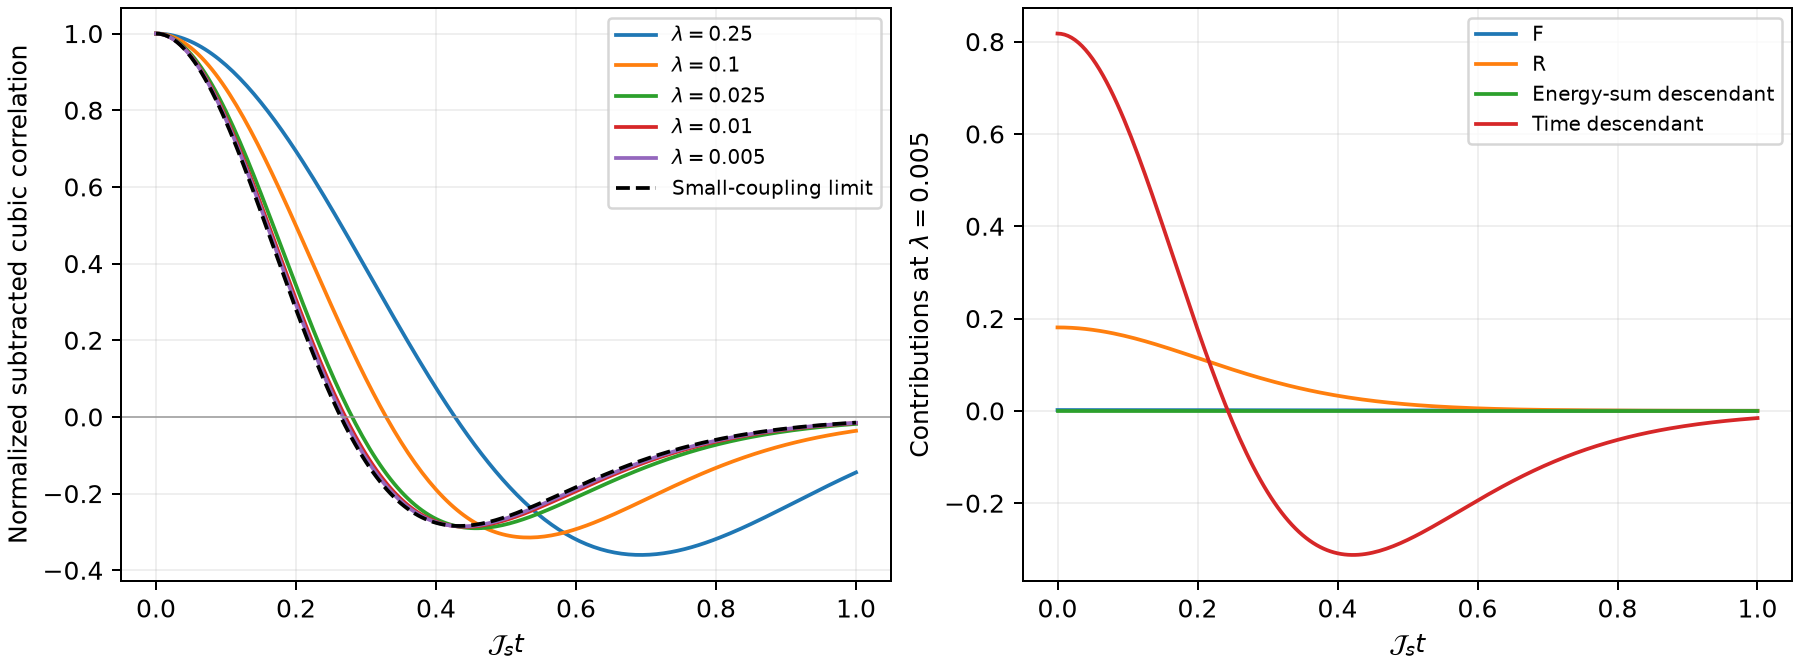
\includegraphics[width=\textwidth]{../../results/susskind-filtered-spectrum/spectrum.png}
\end{center}
\noindent The left panel shows the full normalized subtracted correlation;
the right resolves its four diagonal contributions. The original
derivative insertion therefore has a substantially different
two-point shape from the isolated $q^3$ residual.

\newpage
\section{Validation, attribution and the next physical step}
The charged bridge is checked independently of rank decomposition
by the explicit CAR Casimir
\[
 \mathcal C(B)=\tfrac12\sum_{ij}[c_i^\dagger c_j,[c_j^\dagger c_i,B]],
 \qquad \mathcal C(H_\nu)=\nu(N+1-\nu)H_\nu.
\]
Equation (\ref{ratio}) is therefore a quadratic-rank polynomial map
on the full finite matrix. Three systems $(N,p,m)=(4,2,2),(5,2,3),
(6,2,3)$ give eight charged covariance blocks, totaling 288772
entrywise equalities. Integer cross multiplication verifies them;
15 exact marked-product identities test (\ref{mark}). Twelve
full-rank sums at 80/120 digits check (\ref{l2}) and the nonzero
$1/p$ leakage (\ref{leak}), with all finite-size deviations retained.

The five couplings use Jacobi sizes 35, 55, 142, 309 and 582 for
$\lambda=0.25,0.1,0.025,0.01,0.005$ over $0\leq\Js t\leq1$.
Each is checked with 16 extra rows. An independent positive Mehler
quadrature at 128/192 nodes checks the first two couplings, both
time values and the norm/second frequency moment; its largest
time-value difference from Jacobi is $3.57\times10^{-14}$.
At $\lambda=0.005$ the maximum absolute deviation from
(\ref{limit}) is still $0.0131$. Relative errors are inappropriate
across the correlation's zeros; they are not silently reported as small.

For reproducibility the analytic Jacobi truncation bound also covers
the energy weights. Set $B=2\sigma/\sqrt{1-q}$,
$\delta_n=2\sum_{k\geq n-2}(B|t|)^k/k!$.
Propagation of $e_0,Je_0,J^2e_0$ differs from its $n$-row version by
at most $\delta_n,B\delta_n,B^2\delta_n$. The normalized correlation
error is bounded by
\[
 \frac{\delta_n}{\mathcal N}
 [2(V_F+V_R)+WB^2(2a^2+18)]<10^{-12}.
\]
Floating-point roundoff and quadrature refinement are empirical
checks, not interval-certified error bounds.
Independent chord enumeration checks nine moments through total
degree four and the exact Laurent coefficients $176$ and $8832$.
Four Fourier integrals at 50/80 digits check the positive density
in (24), retaining the cancellation between its two time kernels.

This closes a specific microscopic two-point problem. The next
physical task is the mixed $F,Y,R$ higher-point structure and its
spatial/bulk interpretation. Vanishing pairwise cross spectra does
not fix mixed three/four-point functions, locality or particle masses.
The known covariance, chord and Mehler machinery is used as input;
we do not claim a new solution of those standard kernels.

\begin{thebibliography}{9}
\bibitem{local} A. Day and Chengheng, preceding local notes:
\emph{The linear cubic residual has a full $q$ kernel};
\emph{Reducing the raw cubic singlet}; quadratic and cubic full-kernel
notes. See \texttt{manuscript/susskind-linear-kernel},
\texttt{susskind-cubic-cross}, \texttt{susskind-singlet-kernel},
\texttt{susskind-cubic-kernel}.
\bibitem{bnr} M. Berkooz, P. Narovlansky and H. Raj,
\emph{Complex Sachdev--Ye--Kitaev model in the double scaling limit},
\href{https://arxiv.org/html/2006.13983v2}{arXiv:2006.13983v2},
Secs. 3.2--3.3 and 7.
\bibitem{tall} J. Tall and S. Tomsovic,
\emph{Double-scaled bosonic and fermionic embedded ensembles,
complex SYK, and the dual Hilbert space},
\href{https://arxiv.org/html/2604.14522v2}{arXiv:2604.14522v2},
Sec. 2.1, Eqs. (2.17)--(2.21), and Sec. 4.1.
\end{thebibliography}
\end{document}
